% Options for packages loaded elsewhere
\PassOptionsToPackage{unicode}{hyperref}
\PassOptionsToPackage{hyphens}{url}
%
\documentclass[
  12pt,
]{article}
\usepackage{amsmath,amssymb}
\usepackage{lmodern}
\usepackage{iftex}
\ifPDFTeX
  \usepackage[T1]{fontenc}
  \usepackage[utf8]{inputenc}
  \usepackage{textcomp} % provide euro and other symbols
\else % if luatex or xetex
  \usepackage{unicode-math}
  \defaultfontfeatures{Scale=MatchLowercase}
  \defaultfontfeatures[\rmfamily]{Ligatures=TeX,Scale=1}
\fi
% Use upquote if available, for straight quotes in verbatim environments
\IfFileExists{upquote.sty}{\usepackage{upquote}}{}
\IfFileExists{microtype.sty}{% use microtype if available
  \usepackage[]{microtype}
  \UseMicrotypeSet[protrusion]{basicmath} % disable protrusion for tt fonts
}{}
\makeatletter
\@ifundefined{KOMAClassName}{% if non-KOMA class
  \IfFileExists{parskip.sty}{%
    \usepackage{parskip}
  }{% else
    \setlength{\parindent}{0pt}
    \setlength{\parskip}{6pt plus 2pt minus 1pt}}
}{% if KOMA class
  \KOMAoptions{parskip=half}}
\makeatother
\usepackage{xcolor}
\usepackage{longtable,booktabs,array}
\usepackage{calc} % for calculating minipage widths
% Correct order of tables after \paragraph or \subparagraph
\usepackage{etoolbox}
\makeatletter
\patchcmd\longtable{\par}{\if@noskipsec\mbox{}\fi\par}{}{}
\makeatother
% Allow footnotes in longtable head/foot
\IfFileExists{footnotehyper.sty}{\usepackage{footnotehyper}}{\usepackage{footnote}}
\makesavenoteenv{longtable}
\setlength{\emergencystretch}{3em} % prevent overfull lines
\providecommand{\tightlist}{%
  \setlength{\itemsep}{0pt}\setlength{\parskip}{0pt}}
\setcounter{secnumdepth}{-\maxdimen} % remove section numbering
\newlength{\cslhangindent}
\setlength{\cslhangindent}{1.5em}
\newlength{\csllabelwidth}
\setlength{\csllabelwidth}{3em}
\newlength{\cslentryspacingunit} % times entry-spacing
\setlength{\cslentryspacingunit}{\parskip}
\newenvironment{CSLReferences}[2] % #1 hanging-ident, #2 entry spacing
 {% don't indent paragraphs
  \setlength{\parindent}{0pt}
  % turn on hanging indent if param 1 is 1
  \ifodd #1
  \let\oldpar\par
  \def\par{\hangindent=\cslhangindent\oldpar}
  \fi
  % set entry spacing
  \setlength{\parskip}{#2\cslentryspacingunit}
 }%
 {}
\usepackage{calc}
\newcommand{\CSLBlock}[1]{#1\hfill\break}
\newcommand{\CSLLeftMargin}[1]{\parbox[t]{\csllabelwidth}{#1}}
\newcommand{\CSLRightInline}[1]{\parbox[t]{\linewidth - \csllabelwidth}{#1}\break}
\newcommand{\CSLIndent}[1]{\hspace{\cslhangindent}#1}
\usepackage{float}
\usepackage{graphicx}
\usepackage{booktabs}
\linespread{2}
\usepackage{lineno}
\linenumbers
\usepackage{setspace}\doublespacing
\newcommand{\beginsupplement}{ \setcounter{table}{0}     \renewcommand{\thetable}{S\arabic{table}}\setcounter{figure}{0} \renewcommand{\thefigure}{S\arabic{figure}}}
\providecommand{\keywords}[1]{\textbf{\textit{Keywords---}} #1}

\ifLuaTeX
  \usepackage{selnolig}  % disable illegal ligatures
\fi
\IfFileExists{bookmark.sty}{\usepackage{bookmark}}{\usepackage{hyperref}}
\IfFileExists{xurl.sty}{\usepackage{xurl}}{} % add URL line breaks if available
\urlstyle{same} % disable monospaced font for URLs
\hypersetup{
  pdftitle={ Computational models reveal how cleaner fish adjust decisions in a biological market},
  hidelinks,
  pdfcreator={LaTeX via pandoc}}

\title{\large \textbf{Title:} Computational models reveal how cleaner
fish adjust decisions in a biological market}
\usepackage{etoolbox}
\makeatletter
\providecommand{\subtitle}[1]{% add subtitle to \maketitle
  \apptocmd{\@title}{\par {\large #1 \par}}{}{}
}
\makeatother
\subtitle{\normalsize \textbf{Abbreviated title:} Cleaner fish cognitive
mechanisms in a biological market}
\date{}

\usepackage{forarray}
\usepackage{xstring}
\newcommand{\getIndex}[2]{
  \ForEach{,}{\IfEq{#1}{\thislevelitem}{\number\thislevelcount\ExitForEach}{}}{#2}
}

\newcommand{\getAff}[1]{
  \getIndex{#1}{}
}

\begin{document}
\maketitle
\begin{flushleft}
\end{flushleft}
\begin{abstract}
While it is generally straightforward to quantify individual performance
in cognitive experiments, identifying the underlying cognitive processes
remains a major challenge. Often, different mechanistic underpinnings
yield similar performances, and Lloyd Morgan's cannon warrants
acceptance of the simpler explanation. Alternatively, when the different
mechanisms interact with environmental conditions, variation in
performance across environments might allow to statistically infer the
mechanism responsible. We illustrate this point by fitting computational
models to experimental data on performance by wild-caught cleaner fish
\emph{Labroides dimidiatus} in an ephemeral reward task, as well as
cleaner and client fish densities from the locations of capture. Using
Bayesian statistics to fit the model parameters to performance data
revealed that cleaner fish most likely estimate future consequences of
an action, while it appears unlikely that the removal of the ephemeral
reward acts as psychological punishment (negative reinforcement).
Incorporating future consequences also yields performances that can be
considered the result of locally optimal decision-rules, in contrast to
the negative reinforcement mechanism. We argue that the combination of
computational models with data is a powerful tool to infer the
mechanistic underpinnings of cognitive performance.
\end{abstract}
\subsection*{Lay summary}
Cleaner fish eat ectoparasites off other fishes, so-called clients. It
regularly happens that two clients seek a cleaner's service
simulatenously. Cleaners benefit from prioritising clients unwilling to
wait, so they can feed on those willing to wait. To make the right
choice, cleaners must somehow ``look'' into the future to anticipate
consequences of current choices. By combining a learning model with
data, we show that cleaners estimate the long-term value of their
actions rather than using simpler heuristics. Estimating long-term value
is a mechanism involved in human foresight.


\keywords{learning, behavior, cleaners, bayesian statisitics, behavioral mechanisms}

\newpage

\hypertarget{introduction}{%
\subsection{Introduction}\label{introduction}}

Often alternative cognitive mechanisms yield similar behavior and/or
cognitive performances. This poses a problem for disentangling the
mechanistic underpinnings of behavior. This is particularly clear in
research aimed at discovering between species variation in \emph{higher}
cognitive abilities; or in other words, research on whether non-human
animals show cognitive abilities believed to be uniquely human. For
instance, when researchers try to find \emph{mental time travel-like}
behavior, they usually come up with experiments to show the behavior
displayed requires inferences made through past events (Dally, Emery,
and Clayton 2006). However, they often face the challenge of alternative
scenarios where simpler explanations, like classic associative learning,
can bring about the observed behavioral outcome (Suddendorf and
Corballis 2007). Similarly, attempts to demonstrate the presence of
\emph{theory of mind} in non-human animals face objections justified by
alternative mechanisms underpinning similar behavioral results (C. M.
Heyes 1998). Such controversies are usually settled by using the
principle of parsimony and its cognitive version, Lloyd Morgan's cannon,
which states that the simpler explanation (mechanism) should be
accepted. Ideally, alternative hypotheses should be evaluated in light
of their explanatory power.

Learning is a key overarching cognitive mechanism that allows
individuals to associate rewards with environmental stimuli and thus
behave adaptively (Staddon 2016; Shettleworth 2009). Associative
learning, in particular, exists in all major vertebrate taxa, and in
many invertebrates as well (C. Heyes 2012; Macphail 1982; Staddon 2016;
Behrens et al. 2008). Associative learning is not homogeneous throughout
its taxonomic distribution, rather there are differences across and
within species (Shettleworth 2009; Sih and Giudice 2012). So presumably,
the mechanistic underpinnings of learning have been modified by natural
selection (Marler and Peters 1989).

One way to formalize the alternative mechanistic underpinnings of
associative learning is to develop quantitative models of learning
processes. This approach, which started within experimental psychology
(Staddon 2016; Brandon, Vogel, and Wagner 2002), has been very fruitful
in disentangling the mechanistic structure of cognitive systems. More
recently, the development of reinforcement learning theory (Sutton and
Barto 2018), has allowed to evaluate the empirical support for
alternative mechanistic hypotheses by providing quantitative predictions
which are amenable to statistical tests (Farashahi et al. 2020, 2017).
Interestingly, these learning models not only have received support from
behavioral data, but also are consistent with the current view on reward
processing in the brain (Schultz 2015).

From an evolutionary perspective, mechanisms are likely selected because
of how they allow individuals to respond to environmental variation. For
example, biological market theory predicts that the exchange rate of
goods and/or services traded between cooperative partners adjusts to the
law of supply and demand, when individuals have some degree of partner
choice (Noë and Hammerstein 1995). Supply and demand conditions, which
typically depend on the abundance of the species involved, certainly
vary in time and space. Therefore, natural selection should favor the
ability to flexibly adjust decisions and behavioral output to current
market conditions. Indeed, such adjustments have been documented (Axén,
Leimar, and Hoffman 1996). One example of strategic adjustment in a
biological market is the marine cleaning mutualism involving the cleaner
fish \emph{Labroides dimidiatus} and `client' fishes. Client fishes seek
cleaner fish services at their territory (so-called ``cleaning
station'') and offer themselves as food patches to get their
ectoparasites removed, which provides cleaners with food and clients
with improved health (Waldie et al. 2011; Ros et al. 2011; Triki et al.
2016; Demairé et al. 2020). Given the capacity of some client fish to
swim larger distances and access multiple cleaning stations while others
access the only cleaning station in their territory, it is crucial to
categorize clients as either ``visitors'' or ``residents'',
respectively. During cleaning interactions, a cleaner fish often faces a
choice between a visitor and a resident client seeking its cleaning
services simultaneously. Visitors have the option to switch to another
cleaner fish if being made to wait, while residents must wait for
inspection. Indeed, visitors have been observed to use their partner
choice option in that way (Bshary and Schäffer 2002), which may explain
why cleaners give visitors service priority in a field study in the Red
Sea (Bshary 2001). Furthermore, in a lab based paradigm, design to mimic
the resident-visitor choice (ephemeral reward task), cleaners learned to
prefer the cue associated with the epheral food source (visitor) and
hence accessed both food sources, obtaining double the amount of food
(Bshary and Grutter 2002). However, further exploration revealed that
not all cleaner fish manage to develop a preference for the ephemeral
option in the lab (Triki et al. 2018). Over the last decade, over a
hundred wild-caught cleaner fish have been tested in the exact same
paradigm of the ephemeral reward task (Salwiczek et al. 2012; Wismer et
al. 2014; Triki et al. 2018, 2019, 2020). These fish often come from
different reef locations. Investigation of the local eco-sociological
conditions revealed that cleaner and client fish population densities
have a substantial impact on cleaner fish performance in the task.
Cleaner fish from reef sites with relatively low densities were more
likely to fail at solving the task (Triki et al. 2019, 2018; Wismer et
al. 2014). This intra-specific variation is unlikely due to local
genetic adaptation, because cleaner fish are open water spawners and the
environmental conditions can vary within the lifespan of a fish.

Mechanistic models explicitly designed to mimic the ephemeral reward
task have shown that the simplest form of associative learning (operant
conditioning) cannot account for a solution to the ephemeral reward task
(Prat, Bshary, and Lotem 2022; Quiñones et al. 2019). Operant
conditioning is a form of associative learning where individuals use
short term reward to associate and choose actions. Such models allow
varying the cognitive tool kit and evaluating which minimal kit is
necessary to solve the task at hand (e.g. Dubois et al. (2021)). To be
able to give visitors priority over residents, cleaners need to be able
to assess a client's value separately for the three possible scenarios
(alone, paired with a fish with the same strategic option, paired with a
fish with the alternative strategic option) (Quiñones et al. 2019). The
ability to distinguish and value one stimulus differently alone from
compound versions of it has been termed configurational learning,
chunking, or segmentation (see references in Prat, Bshary, and Lotem
(2022)). In addition to configurational learning, cleaners also need to
account for the future consequences of current decisions. In the model
by Quiñones et al. (2019), this could be achieved in two non-mutually
exclusive ways: through low temporal discounting of future effects, also
termed `chaining' (Enquist, Lind, and Ghirlanda 2016); and/or through
perceiving a visitor client leaving as psychological punishment (i.e.~as
a negative reinforcer). Chaining is when individuals include in their
valuation of an action the reward effects that this will have in the
future. This is done by combining in a single valuation the reward
obtained in the current time with all the reward that comes after,
discounting for how far in the future reward is accrued. `Chaining' the
reward of these different time steps allows individuals to take actions
that increase the long-term reward at the sacrifice of short term
considerations (Enquist, Lind, and Ghirlanda 2016). Even though,
`chaining' can be readily implemented computationally in learning models
(Enquist, Lind, and Ghirlanda 2016; Sutton and Barto 2018), cognitively
it seems to be a complex adaptation (Suddendorf and Corballis 2007). On
the other hand, using client behavior as a negative reinforcer is, in
principle, easier to implement. Thus, the standard logic of Lloyd
Morgan's cannon demands that operant conditioning as the simpler
explanation is to be accepted by default. Ideally, however, the two
mechanisms should be evaluated in light of how well they explain the
available data. Note that different fields interested in cognition and
decision making use different words to refer to negative reinforcers
(Quiñones et al. 2019; Sutton and Barto 2018). Here, for the sake of
simplicity and clarity, we will use the word `penalty' to refer to this
mechanism which includes a negative reinforcer.

In here we used the field and experimental data to fit the parameters of
a reinforcement learning model to infer the cognitive mechanism that
cleaners use in their interaction with clients. Specifically, our
approach of fitting the computational model to the empirical data aimed
at: (i), determining which mechanism cleaner fish use to incorporate
future consequences of current decisions by testing whether chaining,
penalty, or a combination of both best explains their performance; (ii)
determining whether the two mechanisms differed with respect to the
ecological conditions that are likely to cause high versus low
performance in the ephemeral reward task. Additionally, we assessed
which mechanism yields optimal performance patterns. Relying on the
logic of biological market theory, we predicted that appropriate
performance is to show a high preference for visitors only under high
local cleaner-to-client ratio.

\hypertarget{methods}{%
\subsection{Methods}\label{methods}}

\hypertarget{the-model}{%
\subsubsection{The model}\label{the-model}}

The model consists of a set of individual-based simulations where
individuals, representing cleaner fish, face a series of choices between
two options, which simulate the natural conditions of the cleaning
market. Individuals experience a series of discrete time points in which
they face different `states', defined by the number and category of
client fish (visitor or residents) inviting for cleaning services. There
are six possible states: zero clients, one resident, one visitor,
resident-resident, visitor-visitor, and resident-visitor. The
probability of each state is largely determined by the relative
abundance of cleaner fish, residents and visitors, but to some degree by
cleaner fish choices when it faces the resident-visitor combination.
This is because residents are willing to queue for cleaning service;
while visitors leave the queue (with a certain probability) when made to
wait. Individuals obtain a fixed reward from cleaning a client fish
regardless of the category. Every time individuals face and make a
choice they update the probability of making that same choice. The
update is based on the difference between the expected value and the
obtained reward - the prediction error (\(\delta_t\)) - (Sutton and
Barto 2018; Rescorla and Wagner 1972). Formally, the prediction error is
given by

\begin{equation}
\delta_t = R_t -  V_t(S_t) + \gamma V_t(S_{t+1}) ,
\label{eq:delta}
\end{equation}

where \(R_t\) is the sum different reward sources at time \(t\);
\(V_t(S_t)\) is the estimated value at time \(t\) of the the state faced
by the agent at time \(t\); similarly \(V_t(S_{t+1})\) is the estimated
value of the state to come in the following time-step, \(\gamma\) is the
discount factor for future rewards. When the estimated value of the
current state (\(V_t(S_t)\)) is equal to the sum of short-term (\(R_t\))
and future discounted reward (\(\gamma V_t(S_{t+1})\)) learning stops
for that state. If \(\gamma = 0\) the estimates made by the agent only
capture short-term reward. We assume short-term reward to two
components: positive reward determined by the amount of food obtained
from cleaning a client; and negative reward triggered when by a client
leaving the station without being cleaned. Formally, we let total reward
be given by \(R_t=P_t - \eta_t\). Where \(\eta\) is a parameter of the
model that determines the the size of the negative reward triggered by
unattended clients leaving the station.

The prediction error (Eq. \ref{eq:delta}) is used to update the value of
each one of the states the agent faces, as well as the preference for
the resident and visitor options. The value update is simple the product
of the prediction error and the parameter for the speed of learning
(\(\Delta V(S_t)=\alpha \delta_t\)). The change in preference between
the resident and visitor is given by
\(\Delta (\theta_v-\theta_r)_t=\alpha\delta_t2(1-\pi_v)\), where
\(\theta_i\) represent the preference for one of two options and the
difference captures the total change relative to one another; \(\pi_v\)
corresponds to the current probability of choosing the visitor. \(p_i\)
is determined by applying the logistic function to the difference in
preferences between the two mutually exclusive options
(\(\pi_v=\frac{1}{1+e^{-(\theta_v-\theta_r)}}\)). This amounts to a
preference update that is carried in the direction that leads to more
reward being obtained, given the new information. In the long run, the
probability of choosing a visitor over a resident converges in the
model. To which probability the model will converge depends on the
relative abundance of cleaners, visitors and residents; as well as on
the probability of visitors leaving the cleaning station when made to
wait. Further details of the model implementation can be found in
Quiñones et al. (2019).

The model shows that agents need to find a way to incorporate future
consequences of current choices. In the model, this could be achieved
with either of two parameters that could also work together. First,
\(\gamma\) measures how much individuals include future rewards in their
decision updates. If \(\gamma=0\), individuals only use the immediate
reward obtained from a cleaning interaction. As \(\gamma\) increases,
individuals include more of the reward obtained from the subsequent
choices. That amounts to estimating and using for decision making the
future expected rewards of an action (chaining). Second, \(\eta\)
measures how much individuals include in their reward the fleeing
behavior of visitors as a negative component (penalty). Both of these
parameters allow individuals to use in their estimates the future
effects of their choices.

\hypertarget{empirical-data}{%
\subsubsection{Empirical data}\label{empirical-data}}

The empirical data were collected between 2010 and 2019 always during
the austral winter months June to August from a total of five study reef
sites (Corner Beach-CB, Horseshoe-HS, Mermaid Cove-MC, Northern
Horseshoe-NHS, and The Crest-TC) at Lizard Island
(\(14.6682^\circ S, 145.4604^\circ E\)), Great Barrier Reef, Australia.
The data consist of three sets: fish censuses, field observations of
cleaner-client interactions to quantify the probability of visitors
leaving if made to wait, and the performance of wild-caught cleaner fish
in the ephemeral reward test. In total, we have twelve site/year data
sets for fish censuses and corresponding performance in the lab test.
Thus, some sites were sampled more than once. To estimate the population
density of cleaner fish and their clients at a given site in a given
year, Triki et al. (2019) used a series of ten transects of \(30m\)
each. Observers swam along the transect lines placed on the reef and
first counted the visible large-bodied adult fish (species with total
length \(TL \geq 10cm\)) including cleaner fish on a width of \(5m\),
and then on the return individuals of small-bodied fish species
(\(TL < 10 cm\)) on a width of \(1 m\) (see Triki et al. (2018) for
further details on fish censuses data collection). Total length
estimates were done by the observer. We then scaled the counts of
cleaner fish, small-bodied, and large-bodied clients fish densities per
\(100 m^2\).

The field observation data consisted of video recordings/encodings of
the cleaner-client cleaning interactions. There were videos from eight
cleaners per site/year of a duration of \(30 min\) each. Triki et al.~
extracted information from every event wherein a visitor client was made
to wait in favor of another client (visitor or resident), and noted
whether or not the visitor left or queued for the cleaning service
(Triki et al. 2019, 2020).

The cognitive performance data was from a total of 120 cleaners (10
individuals per 12 site/year) tested in the ephemeral reward task (Triki
et al. 2019, 2020). Authors housed all captured cleaners individually in
glass aquaria (\(62cm \times 27cm \times 37 cm\)) and provided them with
PVC pipes (\(10 cm \times 1 cm\)) as shelters. The task consisted of
exposing the cleaner fish to substitute models of client fish in the
form of two \emph{Plexiglas} plates offering the same amount of food
(one item of mashed prawn). The two plates differed in colour and
pattern (horizontal green stripes or vertical pink stripes) but had
equal size (\(10 cm \times 7 cm\)). Importantly, the two plates played
different roles as either a visitor (ephemeral food source) or resident
(permanent food source). That is, if a cleaner fish inspected the
resident plate first, the experimenter withdrew the visitor plate out of
the aquarium as a consequence. Choosing first the visitor plate,
however, granted access to both plates. The equal size of the plates
forced cleaner fish to decide based solely on the association between
the behaviour and the collor/pattern cue (Wismer et al. 2019). Triki et
al. (2019, 2020) tested the fish for a maximum of 200 trials with 20
trials a day, 10 trials in the morning and 10 trials in the afternoon.
They randomized and counterbalanced the plates' spatial location
(i.e.~left or right) between trials. Similarly, they counterbalanced the
plates' decoration (colour and pattern) and the plates' role (visitor or
resident) between the tested fish. In the original studies, once a fish
reached a learning criterion, that is, performing significantly above
chance level in a binomial test (\(p-value \leq 0.05\), ), they passed
to a reversal version of the task where the roles of the
visitor/resident Plexiglas plates were swapped. The reversal phased
stopped when the fish performed significatly above chance, or the fish
completed the 200 trial together with the initial; see Triki et
al.(2019, 2020). Here, we are interested in explaining the total
frequency of visitor choices using the model, rather than just the
achievement of the criterion. Total frequency of visitor choices
naturally comes out of the model, and allows us to use all the variation
among cleaners, instead of reducing that to a binomial variable. Thus,
we used instead a subset of these data to estimate the final cleaner
fish preferences for the visitor plate, even if they do not reach the
learning criterion within 200 trials. To do so, we first extracted the
trial-by-trial outcomes from the last two sessions (20 trials) of those
who never reached the learning criterion for visitor plate (\(N = 45\)
cleaner fish). For those who reached the learning criterion at some
point during the test and passed to a reversal phase, we extracted the
trial-by-trial outcomes from the last session (10 trials) before passing
to reversal and the last 10 trials they were exposed to in the test
(\(N = 75\) cleaner fish).

We chose a combination of initial and reversal to quantify preference
for the visitor client. However, it could be argued that using only the
initial phase gives a better estimation of the cleaner fish preference
for the visitor. In the supplementary material (Fig. \ref{fig:rawdata})
we show how using initial and reversal (a), and only initial (b) maps to
the previously used criteria. The initial and reversal match better the
criteria chosen in previous analysis of the ephemeral reward task
experimental set-up (Triki et al. 2019, 2020).

\hypertarget{statistical-analysis}{%
\subsubsection{Statistical analysis}\label{statistical-analysis}}

The aim of the analyses is to fit the key model parameters \(\gamma\)
and \(\eta\), to the empirical data from Triki et al.~ (2019, 2020) to
test whether each or a combination of these effects is a better
explanation for the pattern seen in the data. We used the ecological
variables: cleaners, visitor clients, resident clients abundances and
visitor clients leaving probability,\\
as input to the models. As the response variable, we used the frequency
with which cleaners chose the visitor option in the ephemeral reward
task. Finally, we used the probability with which agents in the model
simulations choose the visitor in resident-visitor options as the
prediction for the response variable. We kept all other parameter values
used for the model simulations constant, see Table \ref{tab:param}.

To capture with the model the relationship between the ecological
variables and cleaner fish preferences for visitors, we needed to scale
the absolute population densities of cleaner fish from the empirical
data to a measure of relative abundances that captures client visitation
patterns. This is because, in the model, relative abundances of clients
define not only the probability of residents and visitors but also how
often the cleaning station is empty (e.g.~there are no clients to be
cleaned). The frequency with which clients visit the station is another
variable influencing the station occupancy, which in nature may vary
among different client species depending on their ectoparasite loads. We
do not have field estimates for species-specific parasite loads,
especially not as a function of the site. In order to control for these
aspects, we computed a measure of relative cleaner fish abundance for
each reef site relative to absolute abundances and multiplied it by a
scaling constant that changes the range of the variable. Specifically,
cleaner fish relative abundance is equal to
\(\frac{\epsilon C_{abs}}{\epsilon C_{abs}+R_{abs}+V_{abs}}\). Where
\(\epsilon\) is the scaling constant; \(C_{abs}\) is the cleaner fish
absolute density; \(R_{abs}\) is the residents absolute density and
\(V_{abs}\) is the visitor client absolute density. This scaling
constant is meant to capture variation in the market conditions driven
partly by cleaner fish abundance. We fitted the value of the scaling
constant (\(\epsilon\)) as part of the statistical inference. As for the
visitor and resident abundances, we computed a relative measure with
respect to the total client abundance, and weighted that by the
re-scaled relative absence of cleaners
(\(1-\text{relative cleaner abundance}\)). Thus, all three measures of
relative abundance sum up to 1, and can be used in the model as a proxy
for the probability of having different options in the cleaning station.
Note that we introduced the scaling constant to control for variation
that is not captured by the model; its parameter distribution does not
offer biological insights.

Once we calculated the relative abundances, we obtained predictions from
the model for each one of the locations and ran the Markov Chain. We
started the chain with random values for the parameters of interest,
then ran the computational model once for every reef site using as input
the ecological explanatory variables. The model outputs the probability
of choosing the visitor for each location \(p_i\), where \(i\) is the
index for the 12 locations. Assuming a binomial distribution, the
probability that each of the cleaner fish 20 choices in the ephemeral
reward task was generated by the model is given by
\(\binom{n}{k_ij}p^{k_{ij}}_i (1-p_i)^{n-k_{ij}}\); where \(k_{ij}\) is
the number of times that cleaner fish \(j\) in reef site \(i\) chose the
visitor over the resident; and \(n=20\) (due to our choice of using 20
choices per cleaner fish). By taking the natural logarithm and summing
over all the cleaner fish and reef sites, we obtained the log-likelihood
of the data given the model and parameters. We then proposed a new set
of parameters drawn from a uniform distribution centered around the old
parameter set. The amplitude of the uniform distribution used for each
parameter can be found in Table \ref{tab:param}. Subsequently, we ran
the model and calculated the likelihood with the new parameter set. We
then used the ratio of the two likelihoods to choose which parameter set
to keep. New parameter sets with a higher likelihood than the old set
replaced old ones, and those with a lower likelihood replaced current
ones with a probability equal to the log-likelihood ratio. Given that we
only used the likelihoods in the decision, we used an uninformative
prior. Once we decided whether the new parameter set would replace the
old one, we ran the model again to sample the likelihood distribution of
the parameter set. We then started the cycle again by proposing a new
set of parameters and repeated the process for \(1e^5\) steps. We ran 5
independent chains, discarded the first \(1000\) samples of each chain
as burn in, and after that, we kept 1 in every 100 samples to avoid
autocorrelation. The collection of parameters sets kept in all chains
approximates the posterior distribution. We coded the model as well as
the fitting algorithm in \emph{c++}, the diagnostics and visualization
in R (R Core Team 2021). All codes are accessible at
\url{https://zenodo.org/badge/latestdoi/440585701}

To compare the fit of the three alternative models, we used the
distribution of pseudo \(R^2\) proposed by Mcfadden (McFadden 1974).
Mcfadden's pseudo \(R^2\) is a standard measure of fit for logistic
regression. In that context, \(pseudo-R^2\) uses the log-likelihood of
the data given the model, relative to the log-likelihood of the data
given a model without covariates, as a measure of fit. Our model is not
a logistic regression, therefore we measured the \(pseudo-R^2\) in
relation to the log-likelihood of a model with parameters \(\gamma\) and
\(\eta\) set to zero. This, in practice, amounts to a model that has a
neutral preference between the two options. We computed the pseudo
\(R^2\) for all the samples of the posterior from the MCMC. We used
these distributions of pseudo \(R^2\)'s as a measure of fit.

\hypertarget{results}{%
\subsection{Results}\label{results}}

\begin{figure}
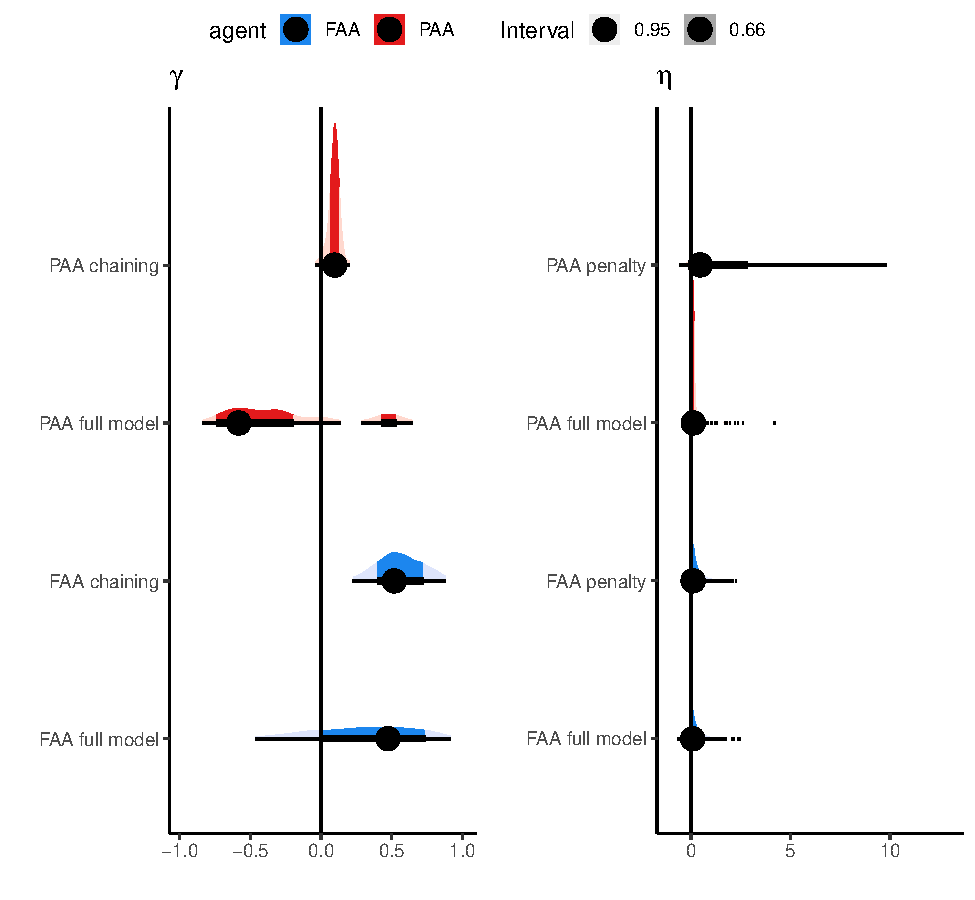
\includegraphics[width=1\linewidth]{manuscript_BE_files/figure-latex/post-1} \caption{Posterior distributions for parameter values $\gamma$ and $\eta$ for the three models (Full model, chaining only and penalty only). We show the kernel density estimates, below the mode (black dot) and the 66 (light blue shade) and 95\% (grey shade)  highest posterior density interval for the two parameters. On the top, panels a and b show posterior distributions for a full model, including chaining ($\gamma$) and penalty ($\eta$). Panel c, shows the $\gamma$ estimate from model with only chaining. Panel d shows the $\eta$ estimate from a model with only penalty. Panel e, shows a measure of fit for all models, namely the distribution of pseudo-$R^2$ obtained from sampling the posterior distribution of parameter values.}\label{fig:post}
\end{figure}

Estimation of parameter values for the three models (full model,
chaining and penalty), support chaining as the only mechanism cleaners
use to account for the future effects of their actions; and thus to
solve the ephemeral reward task. In the estimation of the parameter
values of the full model, which includes both chaining and penalty, the
bulk of the marginal posterior distribution of \(\eta\) which controls
the strength of penalty is around 0 (Fig. \ref{fig:post}). As for
\(\gamma\), controlling chaining, the 95\% confidence intervals also
includes zero, but the mode of the posterior is around 0.5 (Fig.
\ref{fig:post}, a). In the chaining model, where \(\eta\) is set to
zero, the distribution of \(\gamma\) shifted to higher values, zero is
no longer part of the 95\% credible interval of the parameter (Fig.
\ref{fig:post}, c). In contrast, when we look at the model with only
penalty, the posterior distribution of \(\eta\) is still centered around
zero (Fig. \ref{fig:post}, d). Thus, the analysis of the estimates of
individual parameter values in the three models only supports a strong
effect of chaining. Furthermore, the comparison of the models' fit
favors the chaining model. In panel e of figure \ref{fig:post} we show
the distribution of \(pseudo-R^2\) calculated using samples from the
posterior distributions shown before. Note, \(pseudo-R^2\) can have
negative values, which is when the log-likelihood of the model is lower
than that of a model that triggers neutral preferences. Even though the
peak of the three \(pseudo-R^2\) distributions were not very different,
the model with only chaining produced a distribution of \(pseudo-R^2\)
where more values were positive (to the right of the black line in Fig.
\ref{fig:post} e). This shows that accounting for variation in the
parameter estimates the model with chaining gives a better fit to the
data, despite having one parameter less than the full model. We have not
shown here the marginal posterior distributions of the scaling constant,
given that they do not bring biological insight. Their visualizations
can be found in the supplementary material (Fig. \ref{fig:scaConst}), as
well as the diagnostics of the MCMCs (Figs.
\ref{fig:diagnosticsfull},\ref{fig:diaggam},\ref{fig:diagNeg}).

\begin{figure}
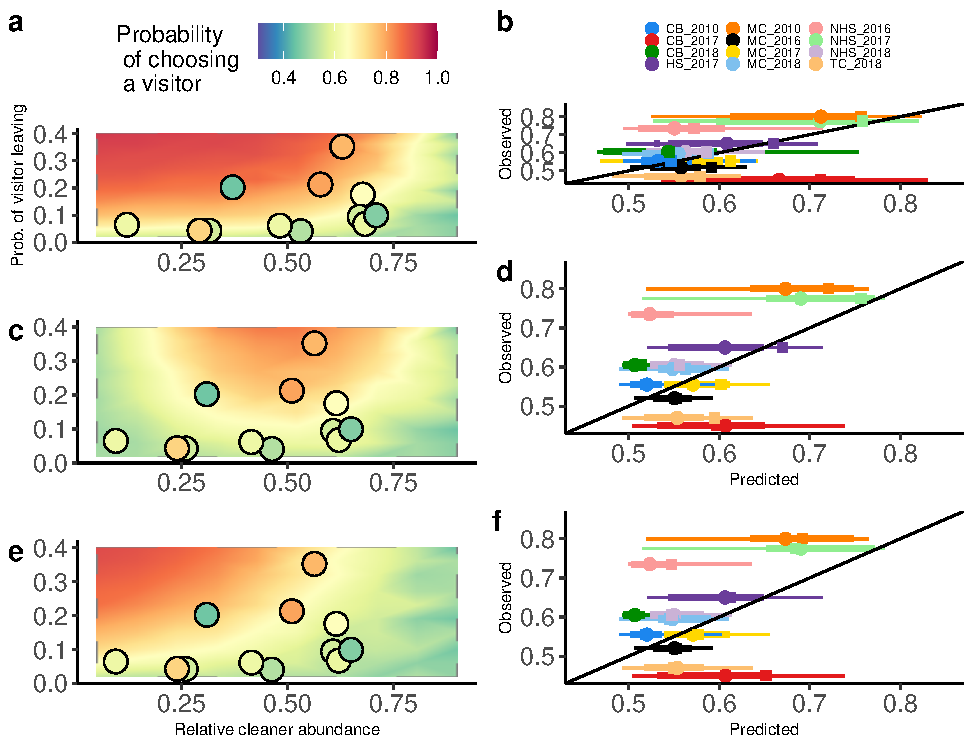
\includegraphics[width=1\linewidth]{manuscript_BE_files/figure-latex/pred-1} \caption{Observed and predicted probability of choosing a visitor. Left-hand side panel: colour contour shows the prediction from the learning model using the mode of the posterior distributions of parameters recovered by the statistical analysis. Dots show the frequency of visitor choices for the 12 reef sites, as well as the corresponding relative cleaner fish abundance (x axis) and frequency of visitors clients leaving the cleaning station (y axis). Right-hand side panels: Variation of the predicted probabilities  of choosing a visitor over a resident and their observed values for 12 locations. Circles show the mean prediction for each location from 100 samples taken from the posterior distribution. Thick and thin bars show the 66 and 95\% credible interval, respectively, taken from those posterior samples. Squares show the predictions used for the panel on the right-hand side. Colour coding denotes different reef site/year of the data collection (see Empirical data section). The black line corresponds to a perfect match between observed and predicted probabilities. Upper panels (a and b) show predictions from a model including chaining and penalty; middle panels (c and d) from a  model with only chaining; lower panels (e and f) from a model with penalty only.}\label{fig:pred}
\end{figure}

Low cleaner fish relative abundance yields different predictions from a
model with only chaining and with penalty. The model with only chaining
predicts a low preference fpr the visitor when cleaner fish relative
abundance is low (Fig. \ref{fig:pred} c). In contrast, the models
including penalty (with and without chaining) predict high preference
for the visitor option (Fig. \ref{fig:pred} a and e). For intermediate
and high cleaner relative abundances the predictions are similar for all
three models. Intermediate relative abundance trigger a high preference
for the visitor; while low abundances trigger low preference for the
visitor (Fig. \ref{fig:pred}a,b,e). Note, however, we calculated
preferences shown in figure \ref{fig:pred} left panels by using only the
model of the posterior distributions, and by holding constant the
balance between resident and visitors' abundances. Panels on the right,
show how close predictions are from the observed data, allowing the
balance between client types to vary and using a set of samples from the
posterior distribution.

Visitor leaving probability has an overall positive effect on the
probability of choosing the visitor clients on all three models. All
three models predict an increase preference for visitors as the visitor
probability increases (Fig. \ref{fig:pred}).

\hypertarget{discussion}{%
\subsection{Discussion}\label{discussion}}

In this study, our main aim was to unravel which of two potential
cognitive mechanisms, chaining of events, penalty, or their combination,
best explains wild-caught cleaner fish performance in the ephemeral
reward task, while accounting for their ecological conditions. To
evaluate the merits of each of these two mechanisms separately and
combined, we considered cleaner fish performance in the lab test to have
its origin from the rule these fish applied in their natural
environment. That is, individuals that solved the task already had a
preference for visitor clients and generalized this rule to the lab
conditions once being familiar with the task.

While all three models captured well the positive relationship between
visitor leaving behavior and cleaner fish performance in the market task
(Triki et al. 2019), only the chaining mechanism predicted that cleaner
fish performance in the task should be low in habitats with low
cleaner-to-client ratios, regardless of the visitor leaving probability.
In contrast, models including negative reward predicted the highest
performance in the ephemeral reward task when relative cleaner fish
abundance is low, particularly together with a high probability of
visitor leaving (Fig. \ref{fig:pred}). Low relative cleaner fish
abundances mean the market has an excess of demand for cleaning
services. In the models, this translates to a cleaning station that is
frequently full. Thus, when a visitor leaves, it is likely that the
cleaner fish will have access to another client in the next step.
Therefore, there will not be much difference in future reward between
choosing a visitor and a resident, and cleaners will not develop a
preference for the visitor in these conditions. On the other hand, the
effect of negative reward on cleaner fish preference is the opposite, as
in a busy cleaning station, to that of chaining. Cleaner fish will get
more often the resident-visitor state and will develop a preference for
the visitor faster. At high cleaner fish abundances, the
resident-visitor state becomes so rare that neither mechanism is very
efficient at generating a preference for visitors. When facing the
resident-visitor choice, it is still best to choose the visitor;
however, the learning machinery will not be able to develop this
preference efficiently. Overall, the models suggest that chaining is the
cognitive mechanism that allows cleaner fish to adaptively adjust to
their biological market ecological conditions.

Previous research showed that cleaner fish living at high population
densities and giving service priority to the visitor plate in the
ephemeral reward task, as well as cleaner fish living at low densities
but denying service priority to the visitor plate possess larger
forebrains; a key teleost brain region associated with behavioural
flexibility and social intelligence. Those failing to show optimized
decision-rules given their local ecological conditions had relatively
smaller forebrains (Triki et al. 2020). Triki et al.~refer to the former
as socially competent cleaner fish, while the second group as socially
incompetent cleaner fish. Social competence is the ability to optimise
social behavior to the available social information (Taborsky and
Oliveira 2012; Bshary and Oliveira 2015; Varela, Teles, and Oliveira
2020). Our analyses yielded no evidence that the difference in social
competence with respect to the local ecological conditions and
associated brain morphology, found by Triki et al. (2020), is due to the
mechanism used to incorporate future consequences. It is conceivable
that high performing individuals from low population densities reef
sites use negative reinforcement instead of chaining, but in that case,
negative reinforcement should have explained at least part of the data.
Configurational learning or chunking (Sutherland and Rudy 1989; Miller
1956), the second component necessary to solve the ephemeral reward task
(Quiñones et al. 2019), was not varied in the models we analysed here.
However, while chunking tendencies should vary to allow individuals to
adapt to their local conditions (Prat, Bshary, and Lotem 2022; Kolodny,
Edelman, and Lotem 2014), systematic differences in individual chunking
tendencies would not explain how socially competent decisions vary as a
function of relative abundance. Therefore, it remains currently unclear
what cell-demanding mechanisms may cause variation in social competence
that translates into site-specific variation in performance in the
ephemeral reward task.

Our models are inspired by the general processes of associative learning
where short term rewards are translated into decision making; thus, it
ignores alternative channels of information that could be relevant in
market-like situations. For example, the model does not investigate
whether cleaner fish actually assess the frequency of client visits or a
mean frequency of visitors leaving. The updating learning mechanism for
the development of preferences works on a trial-by-trial basis. In the
model, cleaner fish do not need to assess the actual state of the
market, \emph{i.e.} their abundance, the abundance of residents and
visitors, and client visitation rate as an indicator of demand. They
only need to assess the short-term consequences of their own decisions
on food intake and chain them. Also, for the sake of simplicity, the
model ignores the process by which cleaner fish discriminate residents
and visitor clients. A model that accounts for this discrimination
probably would involve the development of preferences for morphological
or behavioural features that are statistically associated with visitors
or residents. For example, visitors are on average larger than residents
in body size (Bshary 2001), and contrary to residents, they are less
likely to chase a cleaner fish that fails to cooperate and instead
cheats its client by taking a bite of mucus (Bshary and Grutter 2002).
Given these associations, chaining might produce the decision-rule
``choose the larger client and/or the less aggressive client'', which is
not a useful rule in the standard ephemeral reward task.

In conclusion, our study shows that variation in cognitive performance
as a function of the local ecological conditions may set the stage for
the use of mechanistic modelling to identify the cognitive processes
underlying learning in animals. The combination overcomes the
limitations of the general philosophy in animal cognition to apply the
logic of Lloyd Morgen's canon (Occam's razor). Cognitive experiments
with the aim of excluding basic reinforcement learning as a potential
explanation (operant and/or classical conditioning) of performance often
employ one trial experiments requiring animals to solve the task on the
first possible occasion. For example, any theory of mind task needs to
be solved in the first trial in order to exclude fast conditioning (C.
M. Heyes 1998). Similarly, subjects need to solve a social learning task
on the first trial to accept imitation as a mechanism over
stimulus/local enhancement. Such strict conditions are virtually never
met. For example, potato washing by Japanese macaques, an iconic example
of social learning, took several years to spread within the group
(Kawamura 1959), meaning that any learner had been repeatedly exposed to
demonstrations before acquisition. Importantly, Galef (1992) refuted
imitation as a mechanism not simply because of the repeated exposure but
because a (rather qualitative) analysis of the spread of potato washing
across individuals did not follow the prediction based on imitation
learning (see also Hirata, Watanabe, and Masao (2001)). In our case, the
number of trials it took cleaners to learn the solution to the ephemeral
rewards task would never allow excluding an important role of penalty
based on the data alone. However, fitting model predictions to our
comprehensive empirical data set revealed that a more complex mechanism,
estimation of future reward, fits the data better.

\newpage

\hypertarget{supplementary-material}{%
\section{Supplementary material}\label{supplementary-material}}

\beginsupplement

\begin{figure}
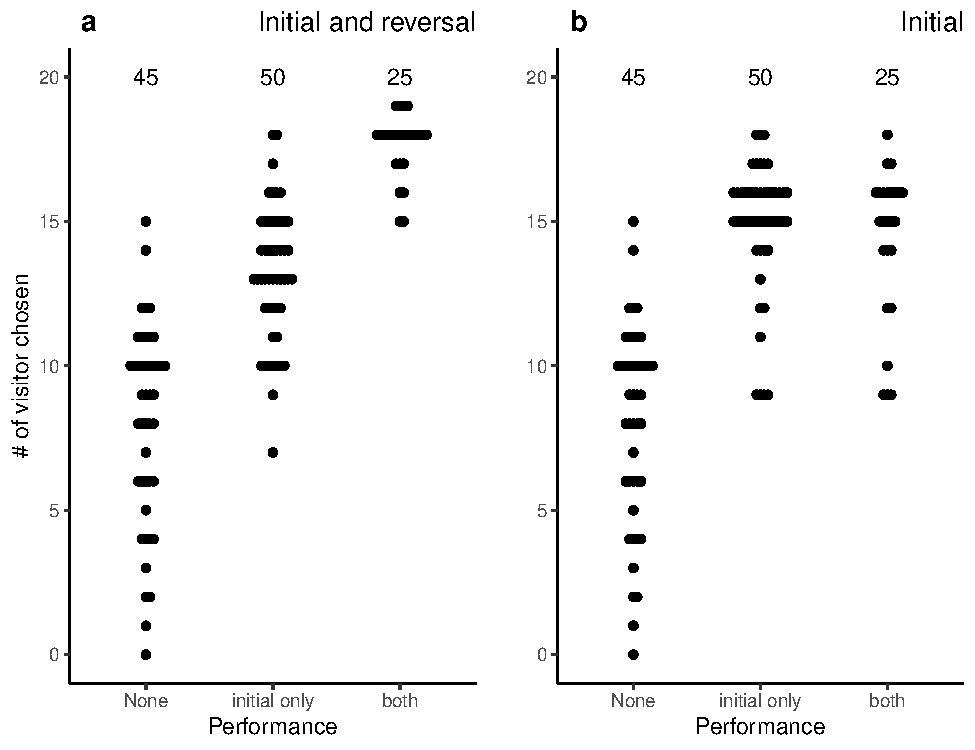
\includegraphics[width=1\linewidth]{manuscript_BE_files/figure-latex/rawdata-1} \caption{Relation between the response variable used in this study and the criteria used in previous studies to assess performance in the ephemeral reward task. In the x axis, we classified the performance of cleaner fish according to whether they developed a preference for the visitor in the initial round (initial only), in the initial and reversal (both), or none of them (none). In the y axis, we add the choices of two experimental sessions: in panel \textbf{a} we use one session from the initial round and one from the reversal round when possible (as described in the main text); in panel \textbf{b} we use two sessions from the initial round for all fish.}\label{fig:rawdata}
\end{figure}

\begin{figure}[H]
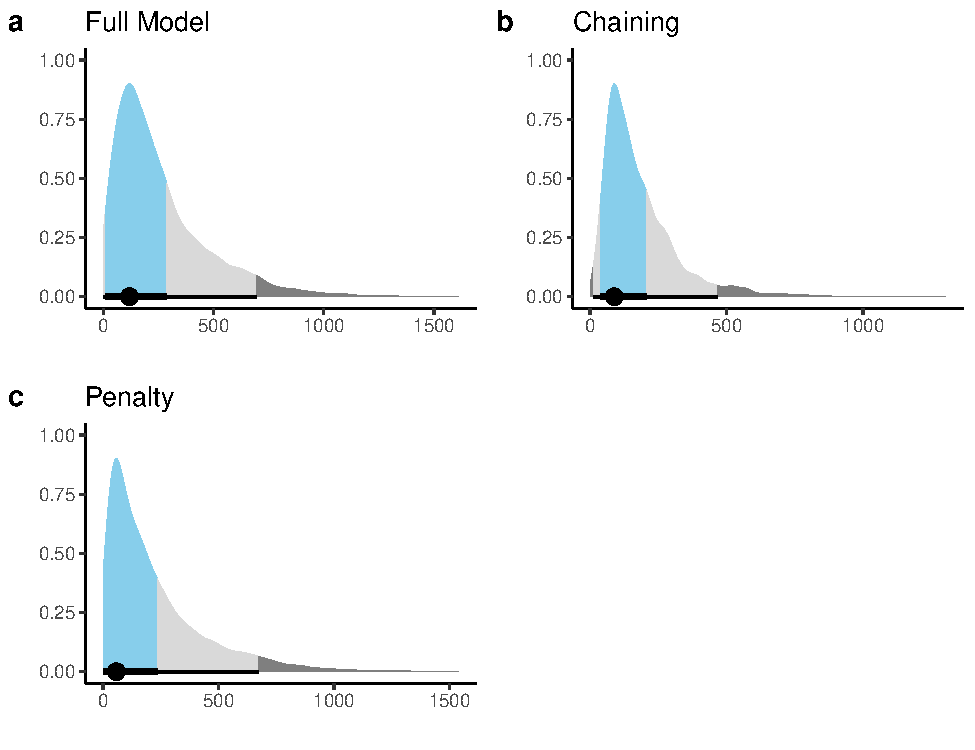
\includegraphics[width=0.95\linewidth,]{manuscript_BE_files/figure-latex/scaConst-1} \caption{Posterior distributions for scaling constant for the three models (Full model, chaining only and penalty only). We show the kernel density estimates, below the mode (black dot) and the 65\% (light blue shade) and 95\% (grey shade)  highest posterior density interval. On the top, panel a shows the posterior distribution from the full model; panel b from the model with only chaining; and panel c from a model with only penalty.}\label{fig:scaConst}
\end{figure}

\begin{figure}
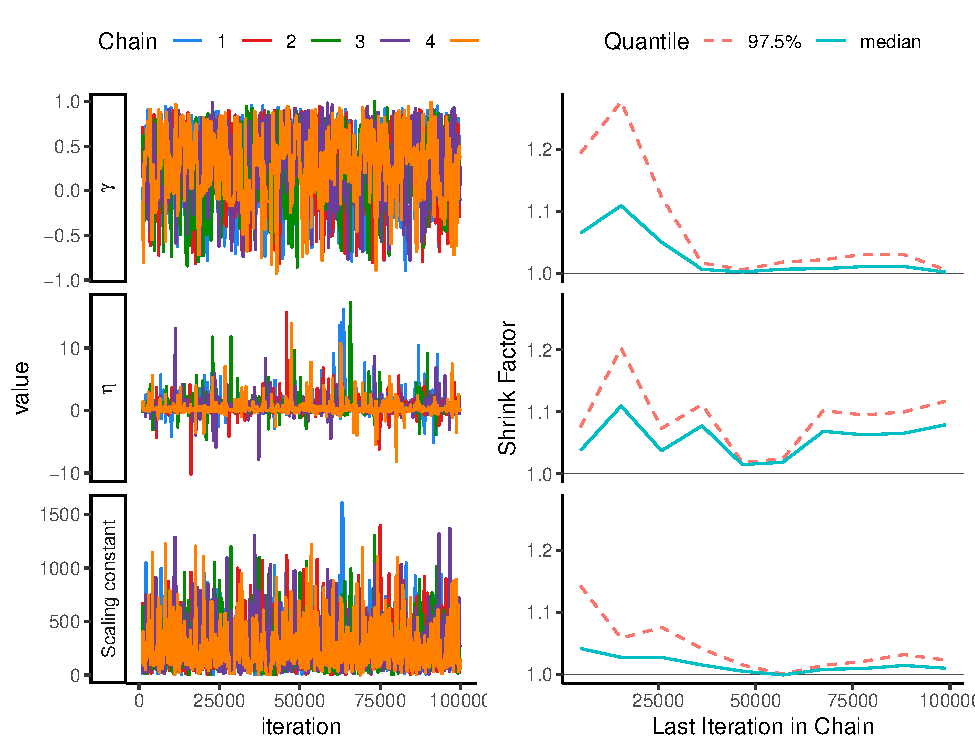
\includegraphics[width=1\linewidth]{manuscript_BE_files/figure-latex/diagnosticsfull-1} \caption{MCMC convergence diagnostics for the full model. On the left trace-plots, on the right changes along the chain of the Gelman and Rubin shrink factor.}\label{fig:diagnosticsfull}
\end{figure}

\begin{figure}
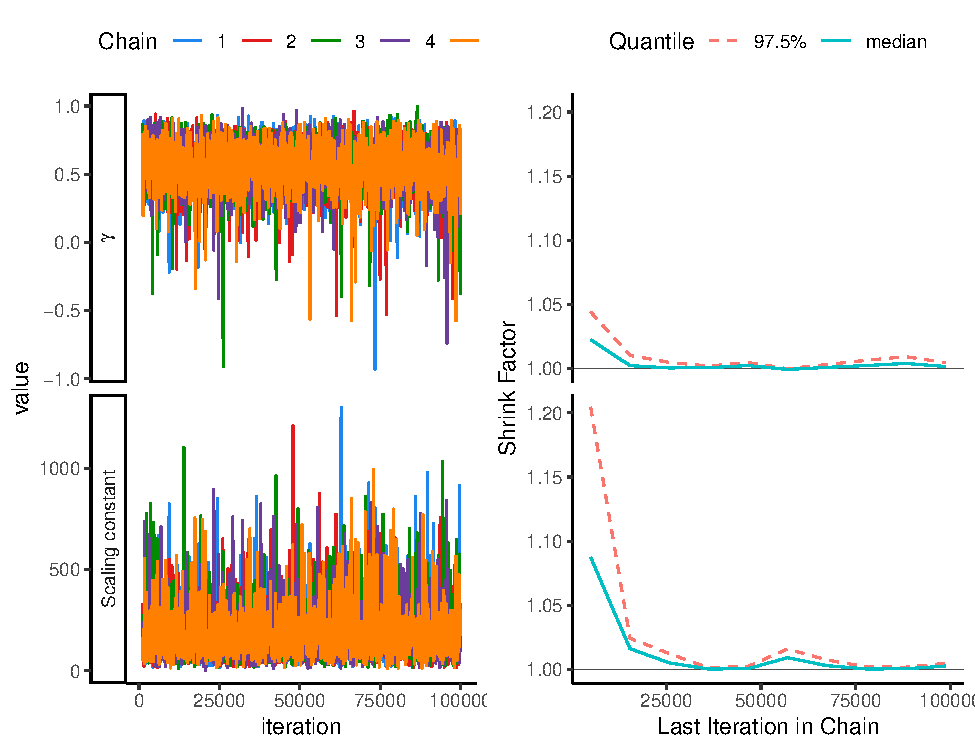
\includegraphics[width=1\linewidth]{manuscript_BE_files/figure-latex/diaggam-1} \caption{MCMC convergence diagnostics for the chaining model. On the left trace-plots, on the right changes along the chain of the Gelman and Rubin shrink factor }\label{fig:diaggam}
\end{figure}

\begin{figure}
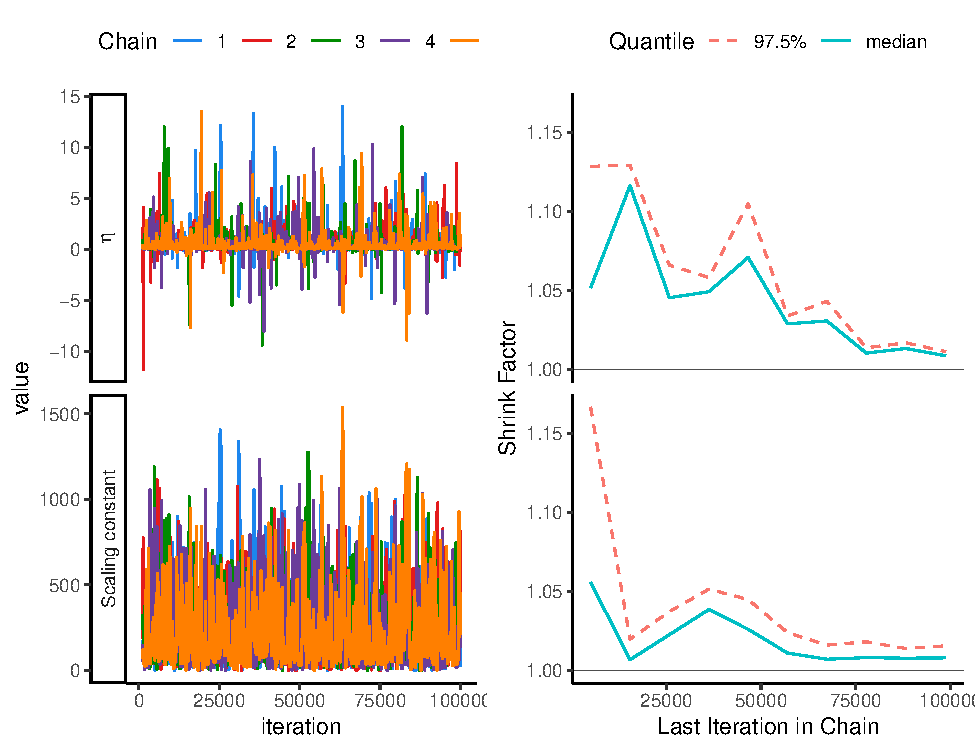
\includegraphics[width=1\linewidth]{manuscript_BE_files/figure-latex/diagNeg-1} \caption{MCMC convergence diagnostics for the penalty model. On the left trace-plots, on the right changes along the chain of the Gelman and Rubin shrink factor}\label{fig:diagNeg}
\end{figure}

\begin{longtable}[]{@{}rc@{}}
\caption{\label{tab:param} Parameter values with which the model was run
in the MCMC. \(\sigma\) refers to the amplitude of the perturbation
kernel with the subscript indicating the associated parameter. New
values were taken from a uniform distribution. \(\alpha\) refers to the
learning rate.}\tabularnewline
\toprule()
Parameter & Value \\
\midrule()
\endfirsthead
\toprule()
Parameter & Value \\
\midrule()
\endhead
Learning rounds & 10000 \\
Reward value & 1 \\
\(\alpha\) & 0.05 \\
\(\sigma_{\gamma}\) & 0.3 \\
\(\sigma_{\eta}\) & 4 \\
\(\sigma_{Sca.Const.}\) & 300 \\
Number of chains & 5 \\
Chain length & \(1^5\) \\
\bottomrule()
\end{longtable}

\hypertarget{references}{%
\section*{References}\label{references}}
\addcontentsline{toc}{section}{References}

\hypertarget{refs}{}
\begin{CSLReferences}{1}{0}
\leavevmode\vadjust pre{\hypertarget{ref-axen_Signalling_1996}{}}%
Axén, Annkristin H., Olof Leimar, and Veronika Hoffman. 1996.
{``Signalling in a Mutualistic Interaction.''} \emph{Animal Behaviour}
52 (2): 321--33. \url{https://doi.org/10.1006/anbe.1996.0178}.

\leavevmode\vadjust pre{\hypertarget{ref-behrens_Associative_2008}{}}%
Behrens, Timothy E. J., Laurence T. Hunt, Mark W. Woolrich, and Matthew
F. S. Rushworth. 2008. {``Associative Learning of Social Value.''}
\emph{Nature} 456 (7219): 245--49.
\url{https://doi.org/10.1038/nature07538}.

\leavevmode\vadjust pre{\hypertarget{ref-brandon_Computational_2002}{}}%
Brandon, Susan E., Edgar H. Vogel, and Allan R. Wagner. 2002.
{``Computational {Theories} of {Classical} {Conditioning}.''} In \emph{A
{Neuroscientist}'s {Guide} to {Classical} {Conditioning}}, edited by
John W. Moore, 232--310. New York, NY: Springer.
\url{https://doi.org/10.1007/978-1-4419-8558-3_7}.

\leavevmode\vadjust pre{\hypertarget{ref-bshary_Cleaner_2001a}{}}%
Bshary, Redouan. 2001. {``The Cleaner Fish Market.''} In \emph{Economics
in {Nature}: {Social} {Dilemmas}, {Mate} {Choice} and {Biological}
{Markets}}, edited by Jan A. R. A. M. Van Hooff, Peter Hammerstein, and
Ronald Noë, 146--72. Cambridge: Cambridge University Press.
\url{https://doi.org/10.1017/CBO9780511752421.010}.

\leavevmode\vadjust pre{\hypertarget{ref-bshary_Asymmetric_2002}{}}%
Bshary, Redouan, and Alexandra S Grutter. 2002. {``Asymmetric Cheating
Opportunities and Partner Control in a Cleaner Fish Mutualism.''}
\emph{Animal Behaviour} 63 (3): 547--55.
\url{https://doi.org/10.1006/anbe.2001.1937}.

\leavevmode\vadjust pre{\hypertarget{ref-bshary_Cooperation_2015}{}}%
Bshary, Redouan, and Rui F Oliveira. 2015. {``Cooperation in Animals:
Toward a Game Theory Within the Framework of Social Competence.''}
\emph{Current Opinion in Behavioral Sciences}, Social behavior, 3
(June): 31--37. \url{https://doi.org/10.1016/j.cobeha.2015.01.008}.

\leavevmode\vadjust pre{\hypertarget{ref-bshary_Choosy_2002}{}}%
Bshary, Redouan, and Daniel Schäffer. 2002. {``Choosy Reef Fish Select
Cleaner Fish That Provide High-Quality Service.''} \emph{Animal
Behaviour} 63 (3): 557--64.
\url{https://doi.org/10.1006/anbe.2001.1923}.

\leavevmode\vadjust pre{\hypertarget{ref-dally_Foodcaching_2006}{}}%
Dally, Joanna M., Nathan J. Emery, and Nicola S. Clayton. 2006.
{``Food-Caching Western Scrub-Jays Keep Track of Who Was Watching
When.''} \emph{Science (New York, N.Y.)} 312 (5780): 1662--65.
\url{https://doi.org/10.1126/science.1126539}.

\leavevmode\vadjust pre{\hypertarget{ref-demaire_Reduced_2020}{}}%
Demairé, Camille, Zegni Triki, Sandra A. Binning, Gaëtan Glauser,
Dominique G. Roche, and Redouan Bshary. 2020. {``Reduced Access to
Cleaner Fish Negatively Impacts the Physiological State of Two Resident
Reef Fishes.''} \emph{Marine Biology} 167 (4): 48.
\url{https://doi.org/10.1007/s00227-020-3658-2}.

\leavevmode\vadjust pre{\hypertarget{ref-dubois_Model_2021}{}}%
Dubois, Thibault, Cristian Pasquaretta, Andrew B. Barron, Jacques
Gautrais, and Mathieu Lihoreau. 2021. {``A Model of Resource
Partitioning Between Foraging Bees Based on Learning.''} \emph{PLOS
Computational Biology} 17 (7): e1009260.
\url{https://doi.org/10.1371/journal.pcbi.1009260}.

\leavevmode\vadjust pre{\hypertarget{ref-enquist_Power_2016}{}}%
Enquist, Magnus, Johan Lind, and Stefano Ghirlanda. 2016. {``The Power
of Associative Learning and the Ontogeny of Optimal Behaviour.''}
\emph{Royal Society Open Science} 3 (11): 160734.
\url{https://doi.org/10.1098/rsos.160734}.

\leavevmode\vadjust pre{\hypertarget{ref-farashahi_Featurebased_2017}{}}%
Farashahi, Shiva, Katherine Rowe, Zohra Aslami, Daeyeol Lee, and Alireza
Soltani. 2017. {``Feature-Based Learning Improves Adaptability Without
Compromising Precision.''} \emph{Nature Communications} 8 (1): 1768.
\url{https://doi.org/10.1038/s41467-017-01874-w}.

\leavevmode\vadjust pre{\hypertarget{ref-farashahi_Learning_2020}{}}%
Farashahi, Shiva, Jane Xu, Shih-Wei Wu, and Alireza Soltani. 2020.
{``Learning Arbitrary Stimulus-Reward Associations for Naturalistic
Stimuli Involves Transition from Learning about Features to Learning
about Objects.''} \emph{Cognition} 205 (December): 104425.
\url{https://doi.org/10.1016/j.cognition.2020.104425}.

\leavevmode\vadjust pre{\hypertarget{ref-galef_Question_1992}{}}%
Galef, Bennett G. 1992. {``The Question of Animal Culture.''}
\emph{Human Nature} 3 (2): 157--78.
\url{https://doi.org/10.1007/BF02692251}.

\leavevmode\vadjust pre{\hypertarget{ref-heyes_Theory_1998}{}}%
Heyes, C. M. 1998. {``Theory of Mind in Nonhuman Primates.''}
\emph{Behavioral and Brain Sciences} 21 (1): 101--14.
\url{https://doi.org/10.1017/S0140525X98000703}.

\leavevmode\vadjust pre{\hypertarget{ref-heyes_Simple_2012}{}}%
Heyes, Cecilia. 2012. {``Simple Minds: A Qualified Defence of
Associative Learning.''} \emph{Philosophical Transactions of the Royal
Society B: Biological Sciences} 367 (1603): 2695--2703.
\url{https://doi.org/10.1098/rstb.2012.0217}.

\leavevmode\vadjust pre{\hypertarget{ref-hirata_SweetPotato_2001}{}}%
Hirata, Satoshi, Kunio Watanabe, and Kawai Masao. 2001.
{``{`{Sweet}-{Potato} {Washing}'} {Revisited}.''} In \emph{Primate
{Origins} of {Human} {Cognition} and {Behavior}}, edited by Tetsuro
Matsuzawa, 487--508. Tokyo: Springer Japan.
\url{https://doi.org/10.1007/978-4-431-09423-4_24}.

\leavevmode\vadjust pre{\hypertarget{ref-kawamura_Process_1959}{}}%
Kawamura, Syunzo. 1959. {``The Process of Sub-Culture Propagation Among
{Japanese} Macaques.''} \emph{Primates} 2 (1): 43--60.
\url{https://doi.org/10.1007/BF01666110}.

\leavevmode\vadjust pre{\hypertarget{ref-kolodny_Evolution_2014}{}}%
Kolodny, O., S. Edelman, and A. Lotem. 2014. {``The Evolution of
Continuous Learning of the Structure of the Environment.''}
\emph{Journal of The Royal Society Interface} 11 (92): 20131091--91.
\url{https://doi.org/10.1098/rsif.2013.1091}.

\leavevmode\vadjust pre{\hypertarget{ref-macphail_Brain_1982}{}}%
Macphail, Euan M. 1982. \emph{Brain and {Intelligence} in
{Vertebrates}}. Clarendon Press.

\leavevmode\vadjust pre{\hypertarget{ref-marler_Species_1989}{}}%
Marler, Peter, and Susan Peters. 1989. {``Species Differences in
Auditory Responsiveness in Early Vocal Learning.''} In \emph{The
Comparative Psychology of Audition: {Perceiving} Complex Sounds},
243--73. Hillsdale, NJ, US: Lawrence Erlbaum Associates, Inc.

\leavevmode\vadjust pre{\hypertarget{ref-mcfadden_Conditional_1974}{}}%
McFadden, Daniel. 1974. {``Conditional Logit Analysis of Qualitative
Choice Behavior.''} \emph{Frontiers in Econometrics}, Frontiers in
econometrics. - {New} {York} {[}u.a.{]} : {Academic} {Press}, {ISBN}
0-12-776150-0. - 1974, p. 105-142,.

\leavevmode\vadjust pre{\hypertarget{ref-miller_Magical_1956}{}}%
Miller, George A. 1956. {``The Magical Number Seven, Plus or Minus Two:
{Some} Limits on Our Capacity for Processing Information.''}
\emph{Psychological Review} 63 (2): 81.

\leavevmode\vadjust pre{\hypertarget{ref-noe_Biological_1995a}{}}%
Noë, Ronald, and Peter Hammerstein. 1995. {``Biological Markets.''}
\emph{Trends in Ecology \& Evolution} 10 (8): 336--39.
\url{https://doi.org/10.1016/S0169-5347(00)89123-5}.

\leavevmode\vadjust pre{\hypertarget{ref-prat_Modelling_2022}{}}%
Prat, Yosef, Redouan Bshary, and Arnon Lotem. 2022. {``Modelling How
Cleaner Fish Approach an Ephemeral Reward Task Demonstrates a Role for
Ecologically Tuned Chunking in the Evolution of Advanced Cognition.''}
\emph{PLOS Biology} 20 (1): e3001519.
\url{https://doi.org/10.1371/journal.pbio.3001519}.

\leavevmode\vadjust pre{\hypertarget{ref-quinones_Reinforcement_2019}{}}%
Quiñones, Andrés E., Olof Leimar, Arnon Lotem, and Redouan Bshary. 2019.
{``Reinforcement {Learning} {Theory} {Reveals} the {Cognitive}
{Requirements} for {Solving} the {Cleaner} {Fish} {Market} {Task}.''}
\emph{The American Naturalist}, December, 000--000.
\url{https://doi.org/10.1086/707519}.

\leavevmode\vadjust pre{\hypertarget{ref-rcoreteam_Language_2021}{}}%
R Core Team. 2021. {``R: {A} Language and Environment for Statistical
Computing.''} Manual. Vienna, Austria. \url{https://www.R-project.org/}.

\leavevmode\vadjust pre{\hypertarget{ref-rescorla_Theory_1972}{}}%
Rescorla, R. A., and A. R. A. Wagner. 1972. {``A Theory of {Pavlovian}
Conditioning: Variations in the Effectiveness of Reinforcement and
Non-Reinforcement.''} In \emph{Classical Conditioning {II}: Current
Research and Theory}, edited by Abraham H. Black and William Frederick
Prokasy. New York: Appleton-Century-Crofts.

\leavevmode\vadjust pre{\hypertarget{ref-ros_Does_2011}{}}%
Ros, Albert F. H., Jeanne Lusa, Meghann Meyer, Marta Soares, Rui F.
Oliveira, Michel Brossard, and Redouan Bshary. 2011. {``Does Access to
the Bluestreak Cleaner Wrasse {Labroides} Dimidiatus Affect Indicators
of Stress and Health in Resident Reef Fishes in the {Red} {Sea}?''}
\emph{Hormones and Behavior} 59 (1): 151--58.
\url{https://doi.org/10.1016/j.yhbeh.2010.11.006}.

\leavevmode\vadjust pre{\hypertarget{ref-salwiczek_Adult_2012}{}}%
Salwiczek, Lucie H., Laurent Prétôt, Lanila Demarta, Darby Proctor,
Jennifer Essler, Ana I. Pinto, Sharon Wismer, Tara Stoinski, Sarah F.
Brosnan, and Redouan Bshary. 2012. {``Adult {Cleaner} {Wrasse}
{Outperform} {Capuchin} {Monkeys}, {Chimpanzees} and {Orang}-Utans in a
{Complex} {Foraging} {Task} {Derived} from {Cleaner} -- {Client} {Reef}
{Fish} {Cooperation}.''} \emph{PLOS ONE} 7 (11): e49068.
\url{https://doi.org/10.1371/journal.pone.0049068}.

\leavevmode\vadjust pre{\hypertarget{ref-schultz_Neuronal_2015}{}}%
Schultz, Wolfram. 2015. {``Neuronal {Reward} and {Decision} {Signals}:
{From} {Theories} to {Data}.''} \emph{Physiological Reviews} 95 (3):
853--951. \url{https://doi.org/10.1152/physrev.00023.2014}.

\leavevmode\vadjust pre{\hypertarget{ref-shettleworth_Cognition_2009}{}}%
Shettleworth, Sara J. 2009. \emph{Cognition, {Evolution}, and
{Behavior}}. 2 edition. Oxford ; New York: Oxford University Press.

\leavevmode\vadjust pre{\hypertarget{ref-sih_Linking_2012}{}}%
Sih, Andrew, and Marco Del Giudice. 2012. {``Linking Behavioural
Syndromes and Cognition: A Behavioural Ecology Perspective.''}
\emph{Philosophical Transactions of the Royal Society of London B:
Biological Sciences} 367 (1603): 2762--72.
\url{https://doi.org/10.1098/rstb.2012.0216}.

\leavevmode\vadjust pre{\hypertarget{ref-staddon_Adaptive_2016}{}}%
Staddon, J. E. R. 2016. \emph{Adaptive {Behavior} and {Learning}}. 2
edition. Cambridge: Cambridge University Press.

\leavevmode\vadjust pre{\hypertarget{ref-suddendorf_Evolution_2007}{}}%
Suddendorf, Thomas, and Michael C. Corballis. 2007. {``The Evolution of
Foresight: {What} Is Mental Time Travel, and Is It Unique to Humans?''}
\emph{The Behavioral and Brain Sciences} 30 (3): 299-313; discussion
313-351. \url{https://doi.org/10.1017/S0140525X07001975}.

\leavevmode\vadjust pre{\hypertarget{ref-sutherland_Configural_1989}{}}%
Sutherland, R. J., and J. W. Rudy. 1989. {``Configural Association
Theory: {The} Role of the Hippocampal Formation in Learning, Memory, and
Amnesia.''} \emph{Psychobiology} 17 (2): 129--44.
\url{https://doi.org/10.3758/BF03337828}.

\leavevmode\vadjust pre{\hypertarget{ref-sutton_Reinforcement_2018}{}}%
Sutton, Richard S., and Andrew G. Barto. 2018. \emph{Reinforcement
{Learning}: {An} {Introduction}}. Edited by Francis Bach. Second edition
edition. Cambridge, MA: A Bradford Book.

\leavevmode\vadjust pre{\hypertarget{ref-taborsky_Social_2012a}{}}%
Taborsky, Barbara, and Rui F. Oliveira. 2012. {``Social Competence: An
Evolutionary Approach.''} \emph{Trends in Ecology \& Evolution} 27 (12):
679--88. \url{https://doi.org/10.1016/j.tree.2012.09.003}.

\leavevmode\vadjust pre{\hypertarget{ref-triki_Brain_2020}{}}%
Triki, Zegni, Yasmin Emery, Magda C. Teles, Rui F. Oliveira, and Redouan
Bshary. 2020. {``Brain Morphology Predicts Social Intelligence in Wild
Cleaner Fish.''} \emph{Nature Communications} 11 (1): 6423.
\url{https://doi.org/10.1038/s41467-020-20130-2}.

\leavevmode\vadjust pre{\hypertarget{ref-triki_Effects_2016}{}}%
Triki, Zegni, Alexandra S. Grutter, Redouan Bshary, and Albert F. H.
Ros. 2016. {``Effects of Short-Term Exposure to Ectoparasites on Fish
Cortisol and Hematocrit Levels.''} \emph{Marine Biology} 163 (9): 187.
\url{https://doi.org/10.1007/s00227-016-2959-y}.

\leavevmode\vadjust pre{\hypertarget{ref-triki_Decrease_2018}{}}%
Triki, Zegni, Sharon Wismer, Elena Levorato, and Redouan Bshary. 2018.
{``A Decrease in the Abundance and Strategic Sophistication of Cleaner
Fish After Environmental Perturbations.''} \emph{Global Change Biology}
24 (1): 481--89. \url{https://doi.org/10.1111/gcb.13943}.

\leavevmode\vadjust pre{\hypertarget{ref-triki_Biological_2019}{}}%
Triki, Zegni, Sharon Wismer, Olivia Rey, Sandra Ann Binning, Elena
Levorato, and Redouan Bshary. 2019. {``Biological Market Effects Predict
Cleaner Fish Strategic Sophistication.''} \emph{Behavioral Ecology} 30
(6): 1548--57. \url{https://doi.org/10.1093/beheco/arz111}.

\leavevmode\vadjust pre{\hypertarget{ref-varela_Correlated_2020}{}}%
Varela, Susana A. M., Magda C. Teles, and Rui F. Oliveira. 2020. {``The
Correlated Evolution of Social Competence and Social Cognition.''}
\emph{Functional Ecology} 34 (2): 332--43.
\url{https://doi.org/10.1111/1365-2435.13416}.

\leavevmode\vadjust pre{\hypertarget{ref-waldie_LongTerm_2011}{}}%
Waldie, Peter A., Simon P. Blomberg, Karen L. Cheney, Anne W. Goldizen,
and Alexandra S. Grutter. 2011. {``Long-{Term} {Effects} of the
{Cleaner} {Fish} {Labroides} Dimidiatus on {Coral} {Reef} {Fish}
{Communities}.''} \emph{PLOS ONE} 6 (6): e21201.
\url{https://doi.org/10.1371/journal.pone.0021201}.

\leavevmode\vadjust pre{\hypertarget{ref-wismer_Cuebased_2019}{}}%
Wismer, Sharon, Ana I. Pinto, Zegni Triki, Alexandra S. Grutter,
Dominique G. Roche, and Redouan Bshary. 2019. {``Cue-Based Decision
Rules of Cleaner Fish in a Biological Market Task.''} \emph{Animal
Behaviour}, October.
\url{https://doi.org/10.1016/j.anbehav.2019.09.013}.

\leavevmode\vadjust pre{\hypertarget{ref-wismer_Variation_2014}{}}%
Wismer, Sharon, Ana I. Pinto, Alex L. Vail, Alexandra S. Grutter, and
Redouan Bshary. 2014. {``Variation in {Cleaner} {Wrasse} {Cooperation}
and {Cognition}: {Influence} of the {Developmental} {Environment}?''}
\emph{Ethology} 120 (6): 519--31.
\url{https://doi.org/10.1111/eth.12223}.

\end{CSLReferences}

\end{document}